\documentclass[linenumbers]{aastex631}


\newcommand{\vdag}{(v)^\dagger}
\newcommand\aastex{AAS\TeX}
\newcommand\latex{La\TeX}

\begin{document}

\title{Strong gravitational-wave lensing forecasts}


\author[0000-0002-0786-7307]{test}
\affiliation{test}


\begin{abstract}
This is an abstract
\end{abstract}

\keywords{TODO}


\section{Introduction} \label{sec:intro}


\section{Results}


\begin{figure}
  \centering
  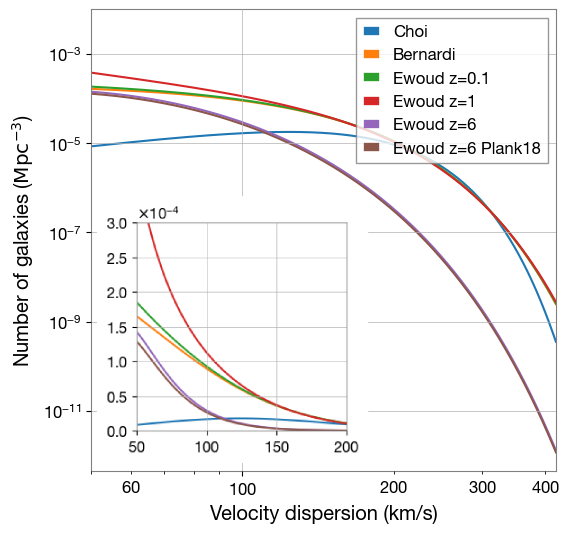
\includegraphics[height=.34\textheight]{figures/velocity_dispersion.png}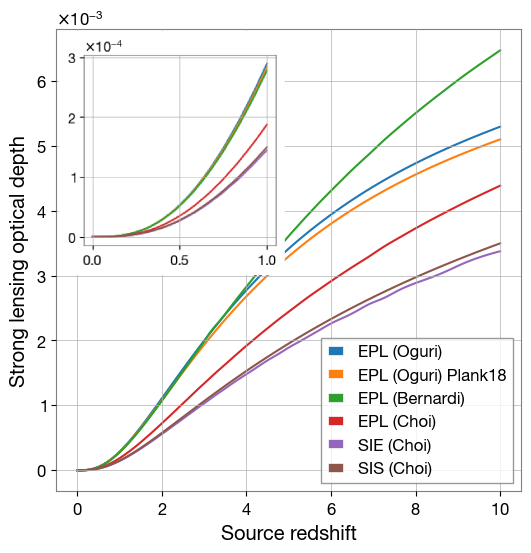
\includegraphics[height=.34\textheight]{figures/optical_depth.png}
  \caption{
    \emph{Left panel:} Number density of galaxies as a function of the velocity dispersion. % Context
    % Content
    The \emph{Choi+2008} distribution (blue) is derived from the SDSS galaxy catalog and includes a fit to the early-type galaxies. 
    The others (Bernardi+2010, Oguri+2018, Wempe+2024) shown in orange, green, red, purple, and brown include all types of galaxies, with slight differences in how the velocity dispersion is modelled as a function of redshift (green to purple) and in the cosmological model choice (brown). 
    The velocity dispersion evolution is derived from a fit to the evolution of the velocity dispersion as predicted by the Illustris simulations; the effect of redshift is illustrated in green to brown. 
    % Conclusion
    The Oguri+2018 and Wempe+2024 reduce to Bernardi+2010 at low redshift because they are extrapolated from the Bernardi local fit to the velocity dispersion profiles. 
    Furthermore, galaxy number density is suppressed at higher redshifts. 
    Finally, the early-type galaxies peak at around 120 km/s. 
    \emph{Right panel:} Strong lensing optical depth as a function of the source redshift. % Context
    % Content 
    The optical depth is estimated from the same models as those used in the left panel. 
    The main differences between the optical depth estimates beyond the model velocity dispersion choice is the lens model choice (spherically symmetric singular isothermal sphere SIS, a singular isothermal ellipsoid SIE, and an elliptical power-law with shear EPL). 
    % Conclusion
    The model choice between an SIS and SIE lens (brown vs purple) does not significantly alter the optical depth (differences at percentage level), 
    while the use of an EPL model with shear has a more significant ($\sim 20-30\,\%$) effect on the optical depth. 
    Furthermore, the choice of the velocity dispersion function has a similar ($\sim 20-50\,\%$) effect, with velocity dispersion profiles with all-type galaxies producing more significant optical depths, and including the suppression of galaxy number densities at high redshift reduces the optical depth. 
    Cosmological model has little effect on either the velocity dispersion profile or the optical depth.
  }
  \label{fig:optical_depth_summary}
\end{figure}


\begin{acknowledgments}
We thank all the people that have made this AASTeX what it is today.  This
includes but not limited to Bob Hanisch, Chris Biemesderfer, Lee Brotzman,
Pierre Landau, Arthur Ogawa, Maxim Markevitch, Alexey Vikhlinin and Amy
Hendrickson. Also special thanks to David Hogg and Daniel Foreman-Mackey
for the new "modern" style design. Considerable help was provided via bug
reports and hacks from numerous people including Patricio Cubillos, Alex
Drlica-Wagner, Sean Lake, Michele Bannister, Peter Williams, and Jonathan
Gagne.
\end{acknowledgments}


\bibliography{bibliography}{}
\bibliographystyle{aasjournal}



\end{document}
